\subsection{Accounting}

The accounting system 
in {\tt DIRAC} is flexible. Refer to figure \ref{fig:acct},
we only need to define 
what a data type is and how this data will be shown.
When a user send a plotting request in the web portal, 
DIRAC will call these methods automatically.
Even though there is a type called {\tt DataOperation} in {\tt DIRAC},
we define our own type. We don't want to mix the data between 
transfer system and the other systems in {\tt DIRAC}.
It is also a try to have our own data type.
\begin{figure}[htbp]
    \begin{center}
\tikzstyle{block} = [rectangle, draw, fill=blue!20, text width=6em, text centered, rounded corners]
\tikzstyle{line} = [draw, -latex, line width=.1em]

\pgfdeclarelayer{background}
\pgfdeclarelayer{foreground}
\pgfsetlayers{background,main,foreground}

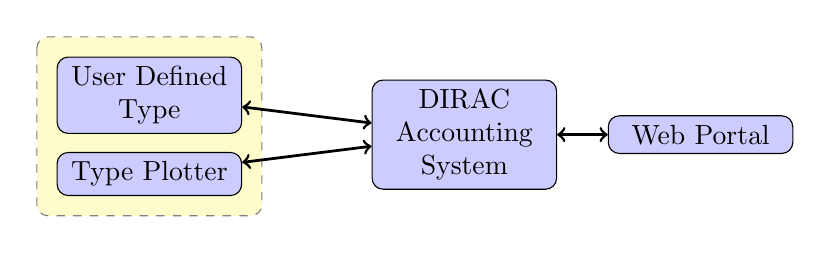
\begin{tikzpicture}[node distance = 2cm, auto]

    % DIRAC Accounting System
    \node [block] (acctkernel) {DIRAC Accounting System};
    % Web Portal
    \node [block, right of=acctkernel, node distance=3cm
            ] (webportal) {Web Portal};

    % vertical line
    \node [left of=acctkernel, node distance=3cm,
            yshift=0.5cm](v1){};
    \node [left of=acctkernel, node distance=3cm,
            yshift=-0.5cm](v2){};

    % user defined type
    \node [block, left of=v1, node distance=1cm, text width=6em,
            ] (usertype) {User Defined Type};
    % type plotter
    \node [block, left of=v2, node distance=1cm, text width=6em,
            ] (plotter) {Type Plotter};

    % Path
    \path[line,<->](usertype)--(acctkernel);
    \path[line,<->](plotter)--(acctkernel);
    \path[line,<->](webportal)--(acctkernel);

    % background
    \begin{pgfonlayer}{background}
        \path (usertype.north west)+(-0.25,0.25) node (g) {};
        \path (plotter.south east)+(0.25,-0.25) node (h) {};
        \path[fill=yellow!20,rounded corners,
        draw=black!50, dashed]
        (g) rectangle (h);
    \end{pgfonlayer}

\end{tikzpicture}
\end{center}


    \caption{\label{fig:acct}DIRAC Accounting System}
\end{figure}
